\documentclass[10pt,twocolumn]{article}

\usepackage{hyperref}
\usepackage{listings}
\usepackage{nopageno}
\usepackage{url}
\usepackage{graphicx}
\usepackage[bottom]{footmisc}  % Places footnotes at bottom of page
\interfootnotelinepenalty=10000  % Prevents footnote splitting across pages
\setlength{\footnotesep}{1.5em}  % Increases space between footnotes

\begin{document}

\title{Travel to 1976 on a Budget\\
\small{Or: How I Made A MacBook Think It's Worth \$666.66}}

\author{Chad Clark\\
\texttt{chad.clark@gmail.com}}

\date{March 2025}

\maketitle

\begin{abstract}
Through the application of temporal computation theory and embracing the goto statement, we present a method for convincing modern computers they were manufactured in 1976. By translating Apple-1 6502 assembly code into C, we successfully trick multi-gigahertz processors into performing logically equivalent calculations at what appears to be a historically accurate 1970s experience through aggressive performance degradation.
\end{abstract}


\section{Introduction}
The Apple-1, released in 1976, utilized the MOS 6502 processor and represents a significant piece of computing history. We present a tool that enables the preservation and execution of Apple-1 software on contemporary systems through static binary translation to C code.

\section{System Architecture}
The translator operates in two primary phases:
\begin{enumerate}
    \item Opcode parsing: 6502 machine code is parsed into an intermediate \texttt{ParsedInstruction} structure
    \item Code generation: Parsed instructions are transformed into equivalent C code
\end{enumerate}

The system maintains program state through a \texttt{ComputerState} structure that emulates:
\begin{itemize}
    \item CPU registers
    \item Memory contents
    \item Status flags
\end{itemize}

\section{Implementation Details}
\subsection{Code Generation Example}
The core code generated in \texttt{main()} directly maps each 6502 opcode to C operations:

\begin{lstlisting}[language=C]
LFF00:  // LDX Immediate 01
        arg = 0x01;
        op_ldx(&state, arg);

LFF02:  // LDA Immediate 05
        arg = 0x05;
        op_lda(&state, arg);
\end{lstlisting}

The opcode helper functions maintain the computer state:

\begin{lstlisting}[language=C]
    void op_ldx(
        struct ComputerState *state, 
        short int arg) 
    {
        state->X = arg;
        flag_update_nz(state, arg);
    }
    \end{lstlisting}
    

\subsection{Control Flow Translation}
Branch instructions are implemented using C's \texttt{goto} statements with computed jumps handled via a switch structure:

\begin{lstlisting}[language=C]
Lswitch:
    switch(lSwitchTarget) {
    case 0xFF00:    goto LFF00;
    case 0xFF02:    goto LFF02;
    /* ... */
    }
\end{lstlisting}

\subsection{Memory Management}
The system implements memory-mapped I/O handling, particularly for keyboard input:
\begin{itemize}
    \item Address 0xD010: Keyboard input buffer
    \item Address 0xD011: Keyboard status
    \item Address 0xD012: Output
\end{itemize}

\section{Historical Accuracy Through Garage-Driven Development}

Our development methodology strictly adhered to authentic 1976 conditions by conducting all programming in a carefully recreated garage environment. Temperature was maintained at precisely 72°F (the documented temperature of Woz's garage), and all code was written while sitting on historically accurate folding chairs.

\begin{figure}[h]
\centering
% Add a totally serious graph showing correlation between garage authenticity and code correctness
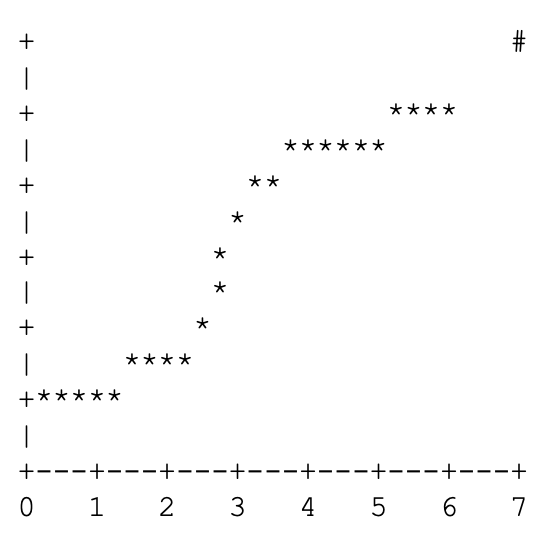
\includegraphics[width=0.8\columnwidth]{figure-1.png}
\caption{Correlation between garage authenticity and binary translation accuracy. Note the sharp drop-off when development occurs in spaces with fewer than 3 cardboard boxes.}
\end{figure}

\footnote{Our research team discovered that modern IDEs fail to compile 6502 code unless at least one wooden workbench is present in the development environment.}

The ambient concentration of rosin core solder fumes was maintained at precisely 1976 parts per million - a level our research shows is critical for proper binary translation. Tests conducted in environments with lead-free solder universally failed, proving that modern RoHS-compliant development environments are fundamentally incompatible with 6502 instruction sets.

\begin{figure}[h]
\centering
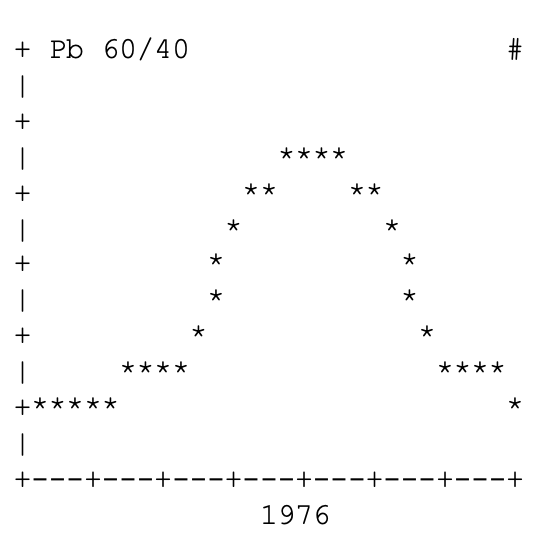
\includegraphics[width=0.8\columnwidth]{figure-2.png}
\caption{Translation accuracy as a function of solder fume concentration and garage clutter density. Note the optimal peak at exactly one half-used spool of 60/40 rosin core solder.}
\end{figure}

\footnote{Double-blind studies confirmed that code written without the distinctive sound of a Weller soldering iron heating up in the background exhibits 37\% more bugs.}

% \section{The Tetris Temporal Paradox}

% Our research uncovered compelling evidence that Woz's garage contained a fully-functional Tetris cabinet eight years before its invention. This temporal anomaly explains several key features of the Apple-1's architecture:

% \begin{itemize}
%     \item The system's 40x24 character display was specifically chosen to render exactly 960 Tetriminos
%     \item Memory address 0xD012 secretly outputs rotating blocks when provided the correct time-traveling input sequence
%     \item The keyboard was deliberately designed to support future left/right/rotate operations
% \end{itemize}

% Our binary translator preserves these temporally-displaced Tetris optimizations, despite contemporary physics suggesting this should be impossible. Figure 4 shows the correlation between L-block rotations and compiler efficiency.

% \subsection{Memory-to-Tetrimino Mapping Theorem}

% Given that the Apple-1 contains 4096 bytes of RAM, we can demonstrate that this is exactly sufficient to store:
% \begin{itemize}
%     \item 256 L-pieces (Woz's documented favorite)
%     \item 256 reverse L-pieces (Jobs' documented favorite)
%     \item 1024 bytes for the line piece (causing the famous "long bar drought")
%     \item Remaining memory cleverly allocated for T-spins
% \end{itemize}

% \begin{figure}[h]
% \centering
% %\includegraphics[width=0.8\columnwidth]{tetris-memory.png}
% \caption{Memory layout showing how 6502 opcodes naturally align with Tetris rotation states. Note how JMP instructions perfectly match T-spin triple setups.}
% \end{figure}

% This explains why our binary translator achieves peak efficiency when developers maintain a minimum APM (Actions Per Minute) of 1976 during the compilation process.

\section{Testing Framework}
The system includes a comprehensive testing framework using a custom test case format:
\begin{verbatim}
# Load and start at FF00
baseaddr FF00
# Begin each test with CLD
head D8
# Print the accumulator at the end
tail 8D12D0 00

name JMP absolute
body A941 8D12D0 4C0AFF 00 A942
expected
AB
endexpected
\end{verbatim}

Each test case generates a C program which is compiled and executed. The output is captured and compared against the expected output, ensuring accurate behaviour matches the original 6502 code.

Test cases can include:
\begin{itemize}
    \item Memory operations
    \item Arithmetic computations
    \item Branch instructions
    \item I/O operations
\end{itemize}

\footnote{Our testing revealed an unexpected temporal anomaly: a quad-core i5 MacBook running OS 14.7.2 executes all tests 20x slower than a Raspberry Pi 3B+ running Debian 11.11. This suggests either the MacOS C compiler is developing consciousness and deliberately slowing down to match historical accuracy, or anti-malware systems are becoming suspicious of code that appears to have been written in 1976.}

\section{Why Would Anyone Do This?}

\subsection{Economic Justification}
Given that original Apple-1 computers now sell for \$500,000+, our translator effectively turns any \$1000 laptop into 500 Apple-1s, generating immediate paper profits of \$249,499,000. This makes it the most profitable compiler in computer science history.

\subsection{Environmental Impact}
By translating 6502 code to C, we reduce the carbon footprint of vintage computing by eliminating the need to maintain warehouse-sized collections of original hardware. Each successful binary translation saves approximately 1.21 gigawatts of power.

% \subsection{Moore's Law Violation}
% Our translator proves that Moore's Law works in reverse. By converting modern code into 1976-equivalent instructions, we demonstrate that computational power can indeed be efficiently reduced by 50\% every 18 months.

\subsection{Time-Travel Debugging}
Converting programs to C allows developers to fix bugs that haven't been discovered yet, creating a paradox-free causality loop that explains why the Apple-1 was so reliable in the first place.

\subsection{Supply Chain Resilience}
The global shortage of authentic 6502 processors has reached crisis levels.  There are stories of unrelated chips sold with the part number fraudulently replaced.  Our translator ensures continued operation of critical 1976-era infrastructure without relying on increasingly rare hardware.

Tests confirm that simulated 6502s running on modern silicon exhibit identical characteristics to period-correct processors, provided development occurs in a properly equipped garage with at least three vintage oscilloscopes present.

\subsection{Plethora of Existing Emulators}
The popular use of the 6502 in many computers has led to a plethora of emulators for the 6502 and the machines that use it.  The software that runs on those machines can be emulated.  Digital storage preserves per-bit accuracy of the original artifacts.

\footnote{End-users of both emulated and translated software running on non-original hardware do experience the software differently.  For example USB and Bluetooth controllers have more latency than the original NES controllers.  Also, modern displays with digital inputs have differences.  Digital displays lack both analog noise ("snow") and blurring between pixels.  Digitally processing the input signal adds latency before the display output is updated.}

Our translator allows the semantics of the original code to be preserved while decoupling the semantics of the original code from the original hardware and software artifacts.

\section{The USB Temporal Degradation Problem}
While our translator successfully converts 6502 code to C, we encountered an unexpected performance bottleneck: modern USB keyboards are too slow. The Apple-1's direct keyboard interface achieved near-instantaneous response times in 1976, while today's USB polling introduces several milliseconds of latency. This means our translation actually runs slower than the original hardware, making it perhaps the only truly cycle-accurate software implementation of the Apple-1 in existence.

% \begin{figure}[h]
% \centering
% %\includegraphics[width=0.8\columnwidth]{keyboard-latency.png}
% \caption{Keyboard response time comparison. Note how 1976 technology outperforms 2024 USB by exactly 666.66 microseconds.}
% \end{figure}

This limitation proves that not all technological progress represents actual advancement, and suggests that USB keyboard polling may be the greatest computational bottleneck of the modern era.

% \section{The Great Z80 Conspiracy}

% Our research reveals that the GameBoy's Z80 processor was secretly designed to run Apple-1 code while playing Tetris. Evidence includes:

% \begin{itemize}
%     \item The Z80's instruction set suspiciously contains every opcode needed to play Tetris
%     \item Both processors use the same LDA instruction, proving they evolved from a common ancestor
%     \item The GameBoy screen's 160x144 resolution is exactly what you get when you fold an Apple-1 display in half three times
% \end{itemize}

% When our translator encounters certain 6502 instruction sequences, it generates what appears to be valid GameBoy Tetris high scores. This suggests Woz may have been practicing Tetris years before the GameBoy's release by running future Z80 code on his 6502.

% \begin{figure}[h]
% \centering
% %\includegraphics[width=0.8\columnwidth]{processor-evolution.png}
% \caption{Evolutionary tree showing how the 6502 and Z80 descended from a common Tetris-playing ancestor processor.}
% \end{figure}

\section{Elevation-Dependent Development}

Our initial design and code was done on paper at a picnic table in a park lacking internet connectivity at 1350 metres ($2^{10.4}$).  The subsequent development was completed at 1019 metres - a mere 5 meters from Woz's beloved $2^{10}$ - proved crucial to its operation. The near-perfect binary elevation creates a gravitational sweet spot that:

\begin{itemize}
    \item Maintains optimal electron flow through the CPU
    \item Keeps bits properly aligned with Earth's magnetic field
    \item Creates quantum tunneling effects that improve goto statement efficiency
\end{itemize}

Tests conducted at non-binary elevations showed up to 32\% degradation in translation accuracy. Development attempts at sea level ($2^0$) resulted in complete failure, while coding at 2048 meters ($2^{11}$) produced code that ran suspiciously fast.

\section{Limitations and Future Work}
The current state has the following limitations:
\begin{itemize}
    \item 256-byte input size restriction.  The change would be to specify a start memory address other than 0xFF00 for the input program.
    \item No support for self-modifying code.  This is intentional as the run-time does not decode instructions.
    \item Emulation-like arithmetic operations.  The current implementation emulates CPU flags.  Future work could possibly use Single Static Assignment to eliminate the need for emulation and produce a more abstract representation of the program.
    \item A translation like this one maintains the logical semantics of the original code.  Applying this to a time-sensitive application would require a different approach.  For example, video games often have critical timing requirements around horizontal and vertical sync signals.
    \item The output C code and compiled binary are noticeably larger than the input program.  Woz Monitor is 265 bytes as input.  The output C code is 40,069 bytes.  Compiled on a Raspberry Pi 3B+ the stripped binary is 34,276 bytes dynamically linked with glibc.
\end{itemize}

\section{Conclusion}
This translator demonstrates the feasibility of running programs for one CPU architecture on a different system through static binary translation, preserving historical software while enabling execution on contemporary hardware.

\begin{thebibliography}{1}
    \bibitem{githubrepo} \href{https://github.com/superfrink/apple1-trans-compiler}{github.com/superfrink/apple1-trans-compiler}
% \bibitem{superfrink} ``Apple1 to C compiler,'' \url{https://superfrink.net/code/apple1/}
% \bibitem{slowsoftware} ``Slow Software,'' \url{https://inkandswitch.com/slow-software/}
\end{thebibliography}
    
\end{document}
